\documentclass[a4paper,12pt]{article}

%Packages to be loaded
\usepackage[fleqn]{amsmath}
\usepackage{amssymb,amsthm}
\usepackage{enumitem}
\usepackage{fancyhdr,url}
\usepackage[english,UKenglish]{babel}
\usepackage{color}
\usepackage{graphicx}

\usepackage{caption}
\usepackage{subcaption}
\graphicspath{{./figures/}}
%Fonts to be loaded
%\usepackage{stmaryrd,bbm}

%Theorem-type declarations

\theoremstyle{definition}
\newtheorem{question}{Question}%[section]
\newtheorem{extnquestion}{Extension Question}[section]
\theoremstyle{remark}
\newtheorem*{problem}{Problem}

%Renew proof text

\renewcommand{\proofname}{Solution:}

%Change style of enumerate's first and second levels

\setenumerate[1]{label=(\alph*),ref=(\alph*)}
\setenumerate[2]{label=\textup{\roman*)},ref=\textup{(\roman*)}}


\date{Version of \today}

%Shortcut commands

%Math:

\newcommand{\bigintersection}{\bigcap}
\newcommand{\bigunion}{\bigcup}
\newcommand{\card}[1]{\lvert #1 \rvert}
\renewcommand{\complement}[1]{{#1}^{\mathrm{c}}}
\newcommand{\cross}{\times}
\newcommand{\curly}[1]{\ensuremath{\mathcal{#1}}}
\newcommand{\defeq}{\stackrel{\scriptscriptstyle{\mathrm{def}}}{=}}
\renewcommand{\epsilon}{\varepsilon}
\newcommand{\integ}{\mathbb{Z}}
\newcommand{\intersection}{\cap}
\newcommand{\midcolon}{}
\newcommand{\nat}{\mathbb{N}}
\renewcommand{\phi}{\varphi}
\newcommand{\reals}{\mathbb{R}}
\newcommand{\surj}{\twoheadrightarrow}
\newcommand{\union}{\cup}

% Functions
\DeclareMathOperator{\Image}{Im}


\pagestyle{fancy}

\selectlanguage{UKenglish}

\dateUKenglish

\begin{document}


%Renew headers, footers
\renewcommand{\headrulewidth}{0pt}
\fancyhead{}
\fancyfoot{}
\cfoot{}
\rfoot{Rhian Davies}

\begin{center} \textbf{{\large Ri Masterclass: A friendly introduction to permutations. }} \\
{\hspace{1em}} \\
\textbf{Exercises}
\end{center}


\begin{question}
 Let $\alpha$ be defined as a permutation such that:

 \begin{align*}
   \label{eq:1}
   \alpha(1) \mapsto 2, \\
   \alpha(2) \mapsto 1, \\
   \alpha(3) \mapsto 4, \\ 
   \alpha(4) \mapsto 5, \\
   \alpha(5) \mapsto 3. \\
 \end{align*}

Draw the permutation $\alpha$ as a permutation diagram.
\end{question}


%\textit{Solution:}
%\\
%\textcolor{white}{.}  \\
%\begin{figure}[h]
%  \centering
%$\alpha$ = 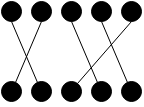
\includegraphics[width = 2.5cm]{5test}.
%
%\end{figure}
\begin{question}
Let \\
\textcolor{white}{.}  \\
%\vspace{2cm}

$\alpha$ = 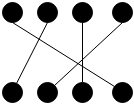
\includegraphics[width = 2cm]{alpha} \qquad and \qquad $\beta$ = 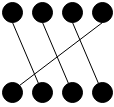
\includegraphics[width = 2cm]{beta}. 

\vspace{1cm}


Find:
\begin{enumerate}
\item $\alpha \circ \beta$,
\item $\beta \circ \alpha$,
\item $\alpha^2$.
\end{enumerate}
\textbf{Reminder: Functions are multiplied from right to left.}
\vspace{0.5em}
\end{question}
%\newpage
%\textit{Solution:}\\
%\textcolor{white}{.}  \\
%$\alpha \circ \beta$ = 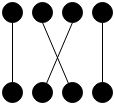
\includegraphics[width = 2cm]{aob}, \\ 
%\textcolor{white}{.} \\
%$\beta \circ \alpha$ = 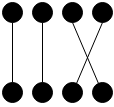
\includegraphics[width = 2cm]{boa},\\ 
%\textcolor{white}{.} \\
%$\alpha \circ \alpha$ = 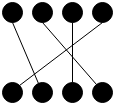
\includegraphics[width = 2cm]{aoa}.\\ 





%\begin{enumerate}
%\item \[ \alpha \circ \beta = \left( \begin{array}{cccc}
%1 & 2 & 3 & 4  \\
%1 & 3 & 2 & 4  \end{array} \right).   \] 

%\item  \[ \beta \circ \alpha = \left( \begin{array}{cccc}
%1 & 2 & 3 & 4  \\
%1 & 2 & 4 & 3  \end{array} \right).   \]

%\item  \[  \alpha^2 = \left( \begin{array}{cccc}
%1 & 2 & 3 & 4  \\
%2 & 4 & 3 & 1  \end{array} \right).   \]
%\end{enumerate}

\clearpage

\begin{question}
Write down all possible permutation diagrams for the set $\left \{ 1\; 2\;3 \right \}$.  
\end{question}

%\textit{Solution:}

%There are six different permutations of the set $\left \{ 1 \;2\;3 \right \}$. 
%
%\begin{figure*}[h!]
%  \centering
%  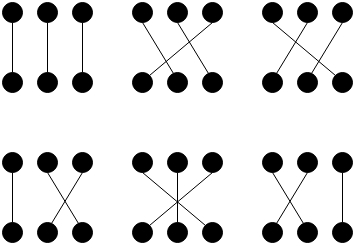
\includegraphics[width = 6cm]{s3.png}
%  \caption{Permutations of the set $\left \{  1\; 2\; 3 \right \}.$}
%\end{figure*}


%\newpage
\begin{question} Every year, Molly Weasley knits Christmas jumpers for her children: Bill, Charlie, Percy, Fred, George, Ron and family friend Harry Potter (excluding Ginny for simplicity). Each jumper is labelled with the first letter of the owners name. 

  \begin{figure}[h]
    \centering
    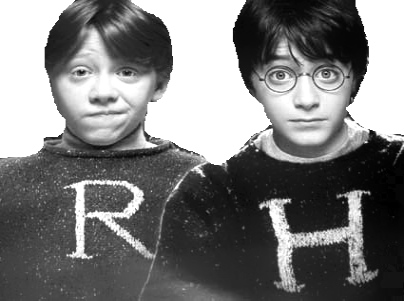
\includegraphics[width = 4cm]{jumper.jpg}
  \end{figure}

  \begin{itemize}
  \item The children put on the correct jumpers in the morning. 
    \item At breakfast, Fred and George swap jumpers. 
      \item At lunch, Charlie swaps jumpers with Bill and Harry swaps jumpers with George.
        \item At teatime, Bill swaps jumpers with Fred, Ron swaps jumpers with Harry and Charlie swaps jumpers with George. 
  \end{itemize}
  \begin{enumerate}
  \item Express these jumper swaps as a permutation diagram. 
    \item Write down the resulting permutation (who is wearing which jumper at the end of the day?)
  \end{enumerate}

\end{question}

%\textit{Solution}: 

%  \begin{figure}[!h]
%    \centering
%    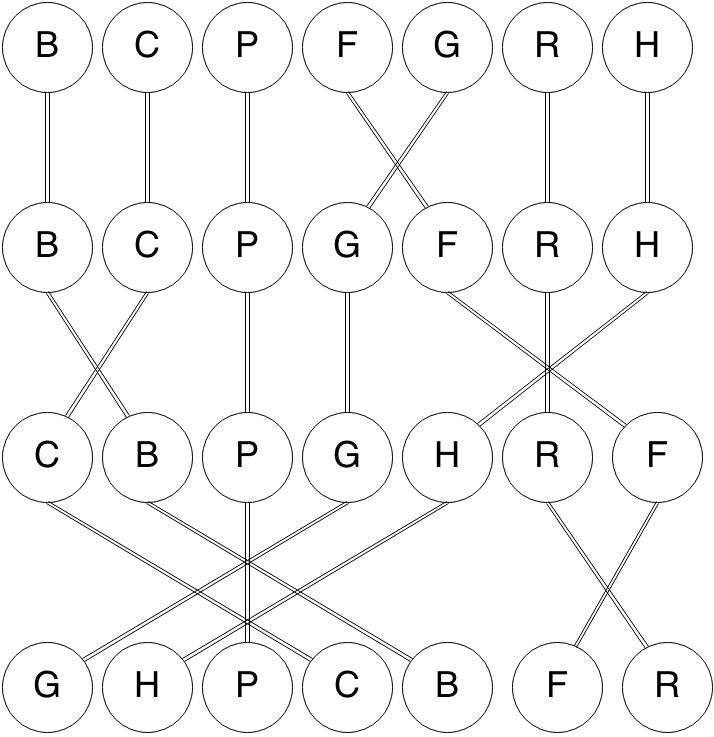
\includegraphics[width = 10cm]{WeasleyJumpers.png}
%  \end{figure}

%Bill is wearing George's jumper, Charlie is wearing Harry's jumper, Percy is wearing his own jumper, Fred is wearing Charlie's jumper, George is wearing Bill's jumper, Ron is wearing Fred's jumper and Harry is wearing Ron's jumper.

\clearpage


\begin{question}

A number of characters from ``The Simpsons'' decide to take part in a Secret Santa. Each character has to buy one gift for another character. Draw the connections in a circle and then write this permutation as a product of disjoint cycles. 
  \begin{table}[h]
\small
    \centering
    \begin{tabular}{|l |l|} \hline
      Participant & Buys for \\ \hline
      Homer &   Bart \\
      Marge & Mr Burns\\
      Bart & Apu\\
      Lisa & Homer\\
      Maggie & Groundskeeper Willie\\
      Mr Burns & Smithers\\
      Smithers & Krusty the Clown\\
      Ned & Marge\\
      Apu &  Lisa\\
      Moe & Maggie\\
      Krusty the Clown & Moe\\
      Groundskeeper Willie &  Ned\\ \hline
    \end{tabular}
  \end{table}
\end{question}

%\textit{Solution:}

%If we number the characters so Homer = 1, Marge = 2, \ldots , Groundskeeper Willie = 12, we can express the permutation as $\alpha = (1\;3\;9\;4)(2\; 6\; 7\; 11\; 10\; 5\; 12\; 8).$ 

% \[ \mbox{Secret Santa} = \left( \begin{array}{cccccccccccc}
%1 & 2 & 3 & 4 & 5 & 6 & 7 & 8 & 9 & 10 & 11 & 12  \\
%3 & 6 & 9 & 1 & 12 & 7 & 11 & 2 & 4 & 5 & 10 & 8 
% \end{array} \right)   \] 

%If we split this up, we get two disjoint cycles. 

%\begin{equation*}
%  \mbox{Secret Santa} = (1\;3\;9\;4)(2\; 6\; 7\; 11\; 10\; 5\; 12\; 8).
%\end{equation*}


%\begin{figure}[h]
%  \centering
%  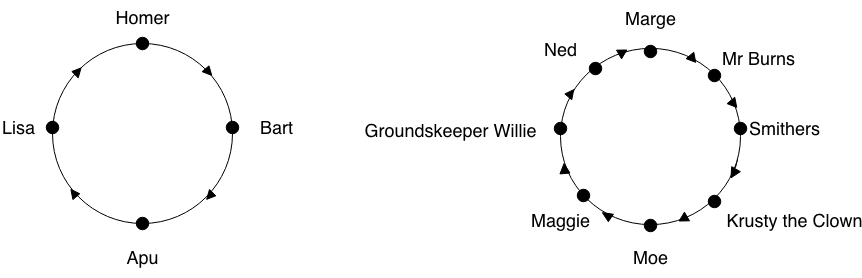
\includegraphics[width = 14cm]{simpson.png}
%\caption{\small{Disjoint cycles for the Simpson's Secret Santa. The symbol $\rightarrow$ means ``Buys a gift for''. }}
%\end{figure}
%\newpage
\begin{question}
  Express each of the following permutations as a single cycle or as the product of disjoint cycles.
  \begin{enumerate}
 \item 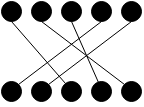
\includegraphics[width = 2cm]{5a}
   \item $\alpha(1) \mapsto 5, \alpha(2) \mapsto 8, \alpha(3) \mapsto 7, \alpha(4) \mapsto 1, \alpha(5) \mapsto 3, \alpha(6) \mapsto 6, \alpha(7) \mapsto 2, \alpha(8) \mapsto 4. $
      \item $(1\;2\;5)(2\;3\;6)$
        \item $(3\;5\;6)(1\;6)(2\;3\;4)$
  \end{enumerate}

\textbf{Reminder: Apply cycles from right to left.}

\end{question}

%\textit{Solution:}

%\begin{enumerate}
%\item $ (1\;3\;4)(2\;5)$
%\item $ (1 \; 5 \;3\;7\;2\;8\;4)$
%\item $(1\;2\;3\;6\;5)$
%\item $(1\;3\;4\;2\;5\;6)$
%\end{enumerate}

\begin{question}
Express $\alpha = (1\;3\;4)(2\;5)$ as a product of transpositions. Can we always represent a cycle as a product of disjoint cycles? Can you prove your answer?
\end{question}

%\textit{Solution:}
%\begin{equation*}
%  \alpha = (1\;3)(3\;4)(2\;5).
%\end{equation*}
%\begin{proof}
%  \begin{equation*}
%    (a_1\;a_2\; \hdots a_k\;) = (a_1\; a_k)(a_1\;a_{k-1})\hdots(a_1\;a_3)(a_1\;a_2).
%  \end{equation*}
%\end{proof}


 


\pagebreak



\end{document}


%%% Local Variables: 
%%% mode: latex
%%% TeX-master: t
%%% End: 


\begin{align*}
&\begin{pmatrix}
1 & 2 & 3    \\
1 & 2 & 3  
\end{pmatrix};
& 
&\begin{pmatrix}
1 & 2 & 3   \\
2 & 3 & 1  
\end{pmatrix};
& 
&\begin{pmatrix}
1 & 2 & 3    \\
3 & 1 & 2 
\end{pmatrix};
\end{align*}

\begin{align*}
&\begin{pmatrix}
1 & 2 & 3    \\
1 & 3 & 2  
\end{pmatrix};
& 
&\begin{pmatrix}
1 & 2 & 3   \\
3 & 2 & 1  
\end{pmatrix};
&
&\begin{pmatrix}
1 & 2 & 3    \\
2 & 1 & 3 
\end{pmatrix}.
\end{align*}


 This can be neated summarised in the permutation below. 
\[ \mbox{Jumper Swap} = \left( \begin{array}{ccccccc}
1 & 2 & 3 & 4 & 5 & 6 & 7  \\
 5 & 7 & 3 & 2 & 1 & 4 & 6\end{array} \right)   \] 


  \item $ \begin{pmatrix}
1 & 2 & 3 & 4 & 5  \\
3 & 5 & 4 & 1 & 2  
\end{pmatrix}$
    \item
     $ \begin{pmatrix}
       1 & 2 & 3 & 4 & 5 & 6 & 7 & 8 \\
       5 & 8 & 7 & 1 & 3 & 6 & 2 & 4 
     \end{pmatrix}$